\subsection{Demostración de la Proposición 1 del enunciado}
Primero observemos que A es una matriz diagonal dominante no estricta. Para eso tenemos que ver que para cada fila el valor absoluto de la diagonal es mayor o igual que la norma-1 del resto de los elementos de esa fila. En nuestro caso puntual, esto significa ver que 
$|c_k| \geq |a_k| + 2|b_k| + |d_k|$\footnote{Los coeficientes están definidos en la sección \ref{sec:armado-sistema}}.

Primero calculemos el lado derecho de la desigualdad:

\begin{eqnarray}
\label{ec:sinModulo}
\left\vert \dfrac{r_k - \Delta r}{r_k (\Delta r)^2}\right\vert +
2 \times \left\vert \dfrac{1}{r_k^2(\Delta \theta)^2} \right\vert+
\left\vert \dfrac{1}{(\Delta r)^2} \right\vert & = &
\dfrac{r_k - \Delta r }{r_k (\Delta r)^2} +
2 \times \dfrac{1}{r_k^2(\Delta \theta)^2} +
\dfrac{1}{(\Delta r)^2}\\ 
& = & 
\label{ec:sinModulo2}
\dfrac{2 r_k^2 (\Delta \theta)^2 - (\Delta r) r_k (\Delta \theta)^2 + 2 (\Delta r)^2}{r_k^2 (\Delta r)^2 (\Delta \theta)^2}
\end{eqnarray}

En (\ref{ec:sinModulo}) efectivamente podemos quitar los módulos pues todos los términos son positivos. Esto es evidente para $b_k$ y $c_k$, aunque un poco menos para $a_k$. En efecto, $r_k - \Delta r$ podría llegar a ser negativo sólo en el caso que $k = 0$, pues $r_k = r_i + k\times \Delta r$. Pero para todos los $t_{0,j}$ no planteamos la ecuación \ref{eq:laplace-discreto} pues ya conocemos su valor, así que no afecta.
 
Entonces, queremos ver que $|b_k|$ es mayor o igual que (\ref{ec:sinModulo2}), es decir

\begin{equation*}
\dfrac{\left\vert -2 r_k^2 (\Delta \theta)^2 + (\Delta r) r_k (\Delta \theta)^2 - 2 (\Delta r)^2 \right\vert } 
{\left\vert r_k^2 (\Delta r)^2 (\Delta \theta)^2 \right\vert } \geq
\dfrac{2 r_k^2 (\Delta \theta)^2 - (\Delta r) r_k (\Delta \theta)^2 + 2 (\Delta r)^2}{r_k^2 (\Delta r)^2 (\Delta \theta)^2}
\end{equation*}

Que es equivalente a

\begin{equation*}
\left\vert -2 r_k^2 (\Delta \theta)^2 + (\Delta r) r_k (\Delta \theta)^2 - 2 (\Delta r)^2 \right\vert \geq
2 r_k^2 (\Delta \theta)^2 - (\Delta r) r_k (\Delta \theta)^2 + 2 (\Delta r)^2
\end{equation*}

Supongamos que lo que está dentro del módulo es positivo, entonces tenemos

\begin{center}
$-2 r_k^2 (\Delta \theta)^2 + (\Delta r) r_k (\Delta \theta)^2 - 2 (\Delta r)^2 \geq
2 r_k^2 (\Delta \theta)^2 - (\Delta r) r_k (\Delta \theta)^2 + 2 (\Delta r)^2$ \\
$\Updownarrow$\\
$2\times (-2 r_k^2 (\Delta \theta)^2 + (\Delta r) r_k (\Delta \theta)^2 - 2 (\Delta r)^2) \geq 0$\\
$\Updownarrow$\\
$-2 r_k^2 (\Delta \theta)^2 + (\Delta r) r_k (\Delta \theta)^2 - 2 (\Delta r)^2 \geq 0$
\end{center}

Pero esta última desigualdad vale pues habíamos supuesto que efectivamente eso era positivo.

Ahora veamos que pasa si lo de adentro del módulo es negativo. Tenemos que 

\begin{center}
$-2 r_k^2 (\Delta \theta)^2 + (\Delta r) r_k (\Delta \theta)^2 - 2 (\Delta r)^2 \leq
-2 r_k^2 (\Delta \theta)^2 + (\Delta r) r_k (\Delta \theta)^2 - 2 (\Delta r)^2$ \\
$\Updownarrow$\\
$0 \leq 0$\\
\end{center}

Que vale trivialmente. Luego probamos que la matriz del sistema es diagonal dominante no estricta, si $~{\left\vert r_k - \Delta r \right\vert \geq 0}$. Notar además que por la última cuenta no es cierto que sea diagonal dominante estricta.


Ahora, la demostración que sigue es similar a la demostración de la proposición que demuestra que diagonal dominante estricta implica que no aparecen ceros en la diagonal al hacer eliminación gaussiana. En esta demostración, simplemente se ve que aplicarle un paso de eliminación gaussiana a la matriz la deja diagonal superior.

Con una lógica muy parecida, podemos ver que la matriz de nuestro problema, luego de aplicarle un paso de eliminación gaussiana, queda diagonal dominante (no estricta). Además, la matriz queda banda, con las bandas exteriores siendo las mismas que antes. Esto se ve claramente, dado que cuando se modifica fila por fila, solo hay que modificar tantas filas como el ancho de la banda, y todas estas filas siguen teniendo la propiedad de tener todos valores iguales a 0 fuera de la banda,
dado que restarle la fila a la que le estamos aplicando el paso de factorización gaussiana tiene todos ceros a partir de un coeficiente.

\begin{figure}[H]
    \begin{center}
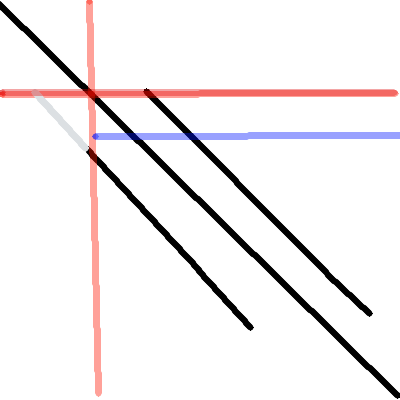
\includegraphics[scale=0.3]{imgs/expl.png}
\end{center}
\caption{\footnotesize{Representación de la matriz, la columna roja indica la columna en la que voy a poner ceros (a la izquierda hay todos ceros, ya que aplicamos eliminación gaussiana), y tengo que restarle la fila roja a la fila azul.}}
 \end{figure}

Luego, vimos que la matriz, al aplicarle un paso de eliminación gaussiana, queda diagonal dominante (no estricta) y banda, con las mismas bandas de siempre. Veamos entonces que la matriz tiene un elemento distinto de 0 en la diagonal, antes de aplicar el siguiente paso de eliminación gaussiana.

Como la fila tiene elementos distintos de 0 (en particular, el coeficiente determinado por la banda superior es siempre distinto de 0), y además la matriz es diagonal superior (no estricta), tenemos que

\[
  |a_{ii}^{(i)}| \geq \sum_{j \neq i} |a_{ij}^{(i)}| > 0
\]

Entonces, $|a_{ii}^{(i)}| > 0$, que es lo que queríamos ver.


